\documentclass{article}

% if you need to pass options to natbib, use, e.g.:
% \PassOptionsToPackage{numbers, compress}{natbib}
% before loading nips_2018

% ready for submission
\usepackage[preprint]{nips_2018}

% to compile a preprint version, e.g., for submission to arXiv, add
% add the [preprint] option:
% \usepackage[preprint]{nips_2018}

% to compile a camera-ready version, add the [final] option, e.g.:
% \usepackage[final]{nips_2018}

% to avoid loading the natbib package, add option nonatbib:
% \usepackage[nonatbib]{nips_2018}

\usepackage[utf8]{inputenc} % allow utf-8 input
\usepackage[T1]{fontenc}    % use 8-bit T1 fonts
\usepackage{hyperref}       % hyperlinks
\usepackage{url}            % simple URL typesetting
\usepackage{booktabs}       % professional-quality tables
\usepackage{amsfonts}       % blackboard math symbols
\usepackage{nicefrac}       % compact symbols for 1/2, etc.
\usepackage{microtype}      % microtypography
\usepackage{graphicx}      % microtypography

\title{Using Neural Speech Recognition Models For Optical Character Recognition
  of Cursive Script}

% The \author macro works with any number of authors. There are two
% commands used to separate the names and addresses of multiple
% authors: \And and \AND.
%
% Using \And between authors leaves it to LaTeX to determine where to
% break the lines. Using \AND forces a line break at that point. So,
% if LaTeX puts 3 of 4 authors names on the first line, and the last
% on the second line, try using \AND instead of \And before the third
% author name.

\author{
  Jon Braatz\\
  \texttt{jfbraatz@stanford.edu} \\
}

\begin{document}
% \nipsfinalcopy is no longer used

\maketitle

\begin{abstract}
  While the tasks of automatic speech recognition (ASR) and optical character
  recognition (OCR) have historically been approached from entirely different
  angles using brittle heuristics and hand-crafted features specific to the task
  at hand, in recent years the most successful models for each task have
  converged on approximately the same neural architectures. The rise of virtual
  assistants like Siri and Alexa has created an incentive for advancing the
  state of the art in voice recognition that is stronger than the incentives in
  the field of OCR, which has led to speech recognition research moving at a
  quicker pace than research in OCR. However, new models used in production like
  Baidu's Deep Speech haven't yet made a mark on the OCR literature, despite the
  fact that the overall structure of models used in both fields are so
  consistently similar. We give heuristic reasons for why the same type of
  end-to-end architecture should give state-of-the-art results for both tasks by
  quantifying structural similarities between the form of thier inputs, and we
  show that Baidu's Deep Speech system can also learn to transcribe written text
  with reasonable accuracy despite not being designed with that task in mind.
\end{abstract}

\section{Introduction}
The recent adoption of deep networks in both the fields of Optical Character
Recognition (OCR) and Automatic Speech Recognition (ASR) have led to a
convergence in the methods used to solve these two tasks. State-of-the art
systems include Google's Tesseract 4 [1] for line recognition in OCR and Baidu's
Deep Speech [2] for transcribing spoken audio clips, and the similarity in their
architectures can be made apparent by considering their pipeline stages:

\begin{enumerate}
\item Preprocess the data to get a clean input that is suitable for the
  transcription task.
  \begin{itemize}
  \item In OCR, this includes binarization, line segmentation, deslanting, etc.
  \item In speech recognition, this can mean applying filters to a raw audio
    signal and converting it to an image by computing its spectrogram.
  \end{itemize}
\item Form the sequence of feature vectors extracted from vertical slices of the
  image using a Convolutional Neural Network.
  \begin{itemize}
  \item Segmentation-free methods that don't explicitly try to learn boundaries
    between semantic units like characters or phonemes are now the most popular
    approaches in both fields.
  \end{itemize}
\item Use a deep Recurrent Neural Network to output probability distributions
  over output characters.
\item Calculate a probability distribution over the complete output sequences
  using the outputs of the RNN and a potentially-multi-step domain model.
  \begin{itemize}
  \item In OCR, the domain model is a language model, which can include n-gram
    statistics of the language, mostly at the character level.
  \item In speech recognition, the domain model would be the language model in
    addition to an accoustic/pronounciation model that accounts for variations
    in tone/pronunciation and thier relative frequencies.
  \end{itemize}
\item Compute Connectionist Temporal Classification (CTC) loss [3] of the output
  sequence and backpropagate.
\end{enumerate}

The fact that both of these state-of-the-art systems are so similar in their
architecture ostensibly speaks to the generality of these kinds of deep neural
networks. However, other state-of-the-art neural NLP systems don't share this
overall structure, so the explanation ``deep networks are applicable to many NLP
contexts'' doesn't explain the reason behind the similarity. Neural Machine
Translation systems, for example, use qualitatively different architectures like
encoder-decoder networks with attention. In particular, NMT systems differ in
that they usually:
\begin{itemize}
\item don't preprocess and encode the input as an image/tensor with meaningful
  continuity in two dimensions.
\item use an embedding-lookup for extracting features from the input sequence
  rather than using a CNN.
\item use an attention mechanism to account for long-range dependencies and
  nonmonotonicity of input-output alignment (``red apple'' $\rightarrow$
  ``manzana roja'')
\item Use cross-entropy loss instead of CTC loss.
\end{itemize}

The specific ways that neural OCR and speech recognition systems differ from NMT
systems clarify which aspects of the OCR and speech recognition problems are
responsible for their solution being so similar. First, the inputs to both
problems are represented in a form that has continuity across two dimensions,
specifically as a more-or-less continuous 2-dimensional signal superimposed on
more-or-less smoothly varying background noise. Second, CNNs are used to extract
features from both of these inputs. Convolutional layers are well-adapted to
text because activations should be equivariant to rigid spatial translations,
and they are well-adapted to speech waveforms because activations should be
equivariant to rigid translations in time (delay) and frequency (pitch).

While ASR and OCR systems are similar, ASR systems often have an additional
language model stage to account for variation in pronunciation, tone of voice,
and context dependence on what was spoken before and after. This additional
model is the acoustic model, a probability distribution for which phoneme is
being pronounced given a short segment of the spectrogram. Additional steps of
this kind are often absent in OCR contexts because OCR systems are usually
optimized for character-based languages, where characters don't change
appearance based on surrounding context. This assumption breaks down for cursive
scripts, like English cursive handwriting or all handwriting and printed text in
Arabic. With these context-sensitive scripts, a character might look completely
different based on its position in a word or surrounding characters. For this
reason, we believe that adapting neural ASR models for OCR will be most
beneficial for cursive scripts that should rightly have a ``grapheme'' model.

\section{Approach and Preliminary Results}
Before moving onto more complicated models based on neural ASR models, we
attained baseline results for a simple model from the SimpleHTC library [4]
comprised of 5 CNN layers, 2 RNN LSTM layers, and CTC loss and decoding. Each CNN
layer consists of a 2D kernel that is either $5 \times 5$ or $3 \times 3$, a
ReLU activation, and a MaxPool operation. This CNN section outputs 32 features
of size 256, which are then fed into a 2-layer RNN with LSTM units with 80
hidden units. The output of the RNN is then fed to the CTC decoder and loss,
which compare with the ground truth transcription.

We trained the model on $20,000$ images in the Arabic Printed Text Image (APTI)
database using Adam optimization and were able to attain a character error rate
of $.704\%$ on the test set and a word accuracy of $96.5\%$, showing that such
an architecture is able to at least recognize the fonts in the dataset. We
haven't attempted data augmentation yet, nor have we moved onto many other fonts
or handwritten text. Data augmentation in the form of random spatial and color
distortions will be done before moving onto more complex models more closely
based on ASR models. However, our results show that cursive scripts like Arabic
are able to be successfully learned by this style of architecture.

We picked Arabic as the script to train on because all Arabic text is cursive,
which means there is much more data available to train on than English cursive,
which isn't commonly typed or written. On the other hand, every possible font
for Arabic is cursive, so in addition to using the APTI database, we could
generate the data ourselves by installing many different Arabic fonts,
generating ground-truth text lines, capturing screenshots of them, and adding
random noise. However, the APTI database has been sufficient so far, and as it
contains text line images from 10 Arabi fonts, each dataset being over 1GB, we
are not yet in danger of running out of data to train on.

\section{Future Work}
The primary future we will undertake is adapt the DeepSpeech architecture for
OCR, in particular DeepSpeech 2 [5], which has a similar architecture to the simple
one used for the baseline. The architecture of the RNN is summarized in Figure
1.

\begin{figure}
  \centering
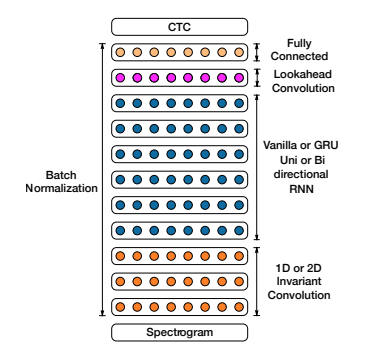
\includegraphics[width=.5\textwidth]{deepspeech2.png}
\caption{Architecture of the deep RNN used in Deep Speech 2}
\end{figure}

In addition to trying to adapt the DeepSpeech architecture for OCR, we plan to
somehow quantify long-range correlations between vertical strips of spectrogram
images and text line images. This will be done to investigate to what extent all
information required to transcribe a character can be localized, and will allow
the two domains of ASR and OCR to be compared to each other. This hasn't been
done yet, but I think it would be nice to have and to compare with long-range
correlations for words as in NMT systems, which are probably longer-range than
correlations between individual character appearance or phoneme pronunciation.


We also plan to train OCR software like Tesseract on spectrograms of human
speech in addition to interpreting text line images as spectrograms and feeding
the associated audio clips into ASR software like DeepSpeech to see how well
each model can train data from the other domain. It could be that the ASR system
component that learns the acoustic model will in this context learn a viable
``grapheme'' model for the cursive script, but we haven't run this experiment
yet.
\section*{References}

\small

[1] Tesseract OCR (https://github.com/tesseract-ocr/tesseract)

[2] Hannun, Awni, Case, Carl, Casper, Jared, Catanzaro, Bryan, Diamos, Greg, Elsen, Erich, Prenger, Ryan, Satheesh, Sanjeev,
Sengupta, Shubho, Coates, Adam, and Ng, Andrew Y. Deep
speech: Scaling up end-to-end speech recognition. 1412.5567,
2014a. http://arxiv.org/abs/1412.5567.

[3] Graves, A., Fernández, S., Gomez, F., and Schmidhuber, J. Connectionist temporal
classification: Labelling unsegmented sequence data with recurrent neural
networks. In ICML, pp. 369– 376. ACM, 2006.

[4] SimpleHTR (https://github.com/githubharald/SimpleHTR)

[5]  Amodei, Dario et al. “Deep Speech 2 : End-to-End Speech Recognition in English and Mandarin.” ICML (2016).

\end{document}